\documentclass[11pt]{article}
\usepackage[margin=1in]{geometry}
\usepackage{lmodern}
\usepackage{amsmath,amssymb,amsthm}
\usepackage{booktabs}
\usepackage{graphicx}
\usepackage{tikz}
\usepackage{pgfplots}
\pgfplotsset{compat=1.18}
\usetikzlibrary{positioning,arrows.meta,calc}
\usepackage{listings}
\usepackage{xcolor}
\usepackage[colorlinks=true,linkcolor=blue,citecolor=blue,urlcolor=blue]{hyperref}
\usepackage{draftwatermark}

\lstset{basicstyle=\ttfamily\footnotesize, language=Python, frame=single,
  breaklines=true, showstringspaces=false, columns=fullflexible,
  keywordstyle=\color{blue!70!black}, commentstyle=\color{green!50!black},
  stringstyle=\color{red!60!black}}

\newtheorem{proposition}{Proposition}
\newtheorem{remark}{Remark}

\definecolor{regfill}{RGB}{225,245,238}
\definecolor{regline}{RGB}{15,110,86}
\definecolor{chord}{RGB}{216,90,48}

\title{An Exact Analytic Derivation of the Polygon Test Boundary\\
for Online Min-Entropy Testing of Binary Data}
\author{David Johnston}

\date{\today}

\begin{document}
\maketitle

\begin{abstract}

This paper replaces the graphical extraction of polygon contours in \cite{johnston2024} 
with a mathematical derivation of the
boundary enabling more accurate min-entropy estimation of binary time series
random data.

A region of count pairs with asymptotic min-entropy rate at least
$H$ is shown to be bounded by exactly two straight lines arising from the
all-ones and all-zeros repeating patterns, one straight feasibility line, and
one curved edge: an arc of an ellipse arising from the alternating
pattern. Closed forms are given for all corner points, for the boundary
equations at any entropy threshold, and for a conservative linear chord that
replaces the elliptic arc with one-sided error. The geometry changes from
a five-sided polygon to a 3 sided triangle (albeit with one edge being the
elliptical arc) when  $H^\ast \geq \log_2\varphi\approx 0.694$, where $\varphi$ is the
golden ratio. Integer comparator constants with conservative
rounding are derived for hardware implementation, along with an integer 
multiplier-based structure that tests the elliptic arc exactly, eliminating
the one-sided error rising from a linear approximation of the arc.
\end{abstract}

\section{Introduction}

The paper\cite{johnston2024} describes an online entropy test (named the 
Polygon Test). By defining mathematical relationships between the counts
of 1s and 1,1 bit pairs in binary time series data with the min-entropy
of the data, a set of polygons is formed on the pattern count plane of 
1s and 11s, where each polygon represents iso-entropy contours. Linear
inequality tests showing the counts lay within a particular iso-entropy
contour allow an efficient hardware or software online entropy test
to be implemented that shows in real time if the min-entropy of a
binary data sequence from a binary random noise source is above
the chosen bound. The polygon is extracted graphically from the
iso-entropy plot which is less than perfectly accurate.

This paper replaces the graphical extraction with a mathematical derivation of the
boundary. 

A two-state Markov model with transition probabilities $P_{01}$ (probability a
0 is followed by a 1) and $P_{10}$ (probability a 1 is followed by a 0) can
generate binary data with any chosen mean $\mu$ and serial
correlation coefficient (SCC), and its min-entropy is computable from the
model parameters~\cite{johnston2024}. That paper further showed that the two
counters
\[
\mathit{count1}=\text{(number of 1s in the first $n-1$ bits)},\qquad
\mathit{count11}=\text{(number of 11 bit pairs)}
\]
over an $n$-bit block carry the same information as the Markov transition
probabilities of a two state Markov generator,
and that the region of count pairs corresponding to min-entropy above a
threshold appears, when plotted, to be a polygon testable with a small number
of linear inequality tests --- the \emph{polygon test}, deployed as the
vendor-defined continuous health test in fifth generation Intel CPU RNGs.

The polygon of~\cite{johnston2024} was extracted from a rendered contour
plot. One edge appeared curved and convex, but it was not established whether
it was piecewise linear or curved, and the corner coordinates carried
image-extraction error. This paper addresses that shortcoming. The boundary in
closed form is derived and it is shown that the curved edge is an arc
of an ellipse. Formulae for exact corner positions are given. A polygon
form transition from five sided to three sided in the boundary at
$H^\ast=\log_2\varphi$ is identified. A set of integer comparator constants
are derived whose rounding
direction ensures the resulting test error is one-sided and so is conservative.

\section{Count Coordinates and the Inverse Map}
\label{sec:inverse}

For this calculation the coordinates are normalized over a block of $n$ bits with $N=n-1$ bit-pair
positions:
\[
x = \mathit{pc1} = \frac{\mathit{count1}}{N} = \hat\mu, \qquad
y = \mathit{pc11} = \frac{\mathit{count11}}{N}.
\]
For the two-state Markov chain, $y$ estimates
$\Pr[x_i{=}1, x_{i+1}{=}1]=\mu P_{11}$ and $x$ estimates $\mu$, so the four
transition probabilities can be recovered from $(x,y)$ as
\begin{equation}
P_{11}=\frac{y}{x},\qquad
P_{10}=1-\frac{y}{x},\qquad
P_{01}=\frac{x-y}{1-x},\qquad
P_{00}=\frac{1-2x+y}{1-x}.
\label{eq:inverse}
\end{equation}
These are the empirical conditional transition frequencies:
$x-y$ is $\mathit{pc10}$ and $1-2x+y$ is $\mathit{pc00}$ (each to within one
count, since $\mathit{count01}$ and $\mathit{count10}$ can differ by at most
one in non-cyclic data), so $P_{11}=\mathit{count11}/\mathit{count1}$ and
$P_{00}=\mathit{count00}/\mathit{count0}$.

\section{The Min-Entropy Rate in Closed Form}
\label{sec:rate}

The most common value (MCV) of a $b$-bit symbol from the model is a repeating
two-bit pattern (all ones, all zeros, or alternating), possibly with a
deviating final bit for even $b$~\cite{johnston2024}. The symbol probabilities
of the MCV candidates have the form
$(\text{prefactor})\cdot P_{11}^{\,b-1}$,
$(\text{prefactor})\cdot P_{00}^{\,b-1}$, or
$(\text{prefactor})\cdot (P_{01}P_{10})^{\lfloor (b-1)/2\rfloor}$,
where the prefactors such as $(P_{01}+P_{11})$ do not grow with $b$.
The per-bit min-entropy rate is therefore determined by the stepwise
geometric growth of the bit pattern of the MCV:
\begin{equation}
H_\infty(x,y)
= -\log_2 \max\!\Bigl(\, P_{11},\; P_{00},\; \sqrt{P_{01}P_{10}} \,\Bigr)
= -\log_2 \max\!\left( \frac{y}{x},\;
\frac{1-2x+y}{1-x},\;
\frac{x-y}{\sqrt{x(1-x)}} \right).
\label{eq:Hrate}
\end{equation}
Equation~\eqref{eq:Hrate} is the exact analytic form of the contours plotted
in Figure~10 of~\cite{johnston2024}. The prefactors shift the finite-width
boundary by $O(1/b)$; for a block-level online test the rate is the right
object, and the finite-width correction is discussed in
Section~\ref{sec:drawbacks}.

\section{The Exact Boundary}
\label{sec:boundary}

Let $p=2^{-H}$ for a chosen threshold $H$. The region
$\mathcal{R}_H=\{(x,y): H_\infty(x,y)\ge H\}$ is the intersection of three
entropy constraints and the parameter feasibility constraints
$0\le P_{01}\le 1$, $P_{11}\ge 0$:
\begin{center}
\begin{tabular}{llll}
\toprule
Constraint & In $(x,y)$ & Shape & Edge name \\
\midrule
$P_{00}\le p$ & $y \le (2-p)\,x - (1-p)$ & straight line & AB \\
$P_{11}\le p$ & $y \le p\,x$ & straight line through origin & BC \\
$P_{01}\le 1$ & $y \ge 2x-1$ & straight line & CD \\
$\sqrt{P_{01}P_{10}}\le p$ & $(x-y)^2 \le p^2\,x(1-x)$ & \textbf{ellipse} & DE \\
$P_{11}\ge 0$ & $y\ge 0$ & axis & EA \\
\bottomrule
\end{tabular}
\end{center}

\begin{proposition}[The curved edge is an ellipse arc]
The constraint $(x-y)^2 \le p^2 x(1-x)$ expands to
$(1+p^2)x^2 - 2xy + y^2 - p^2 x \le 0$, a conic with discriminant
$B^2-4AC = 4-4(1+p^2) = -4p^2 < 0$: an ellipse. The boundary edge is the
lower branch
\begin{equation}
y = x - p\sqrt{x(1-x)}.
\label{eq:arc}
\end{equation}
Since $\sqrt{x-x^2}$ is concave, $x - p\sqrt{x-x^2}$ is convex. The DE edge
is therefore curved and convex, not piecewise linear, confirming
the visual impression in~\cite{johnston2024}. Chords of a convex arc lie above it, so linear
approximations by chords are automatically conservative
(Section~\ref{sec:chord}).
\end{proposition}

Notably, the CD edge $y \ge 2x-1$ used in~\cite{johnston2024} was written
down from the plot but is in fact \emph{exact}: it is the feasibility line
$P_{01}=1$, equivalently $\mathit{count00}=0$ to within one count.

\section{Corners and the Two Regimes}
\label{sec:corners}

Intersecting adjacent constraints yields closed forms for every corner. Two
regimes arise, separated by whether the constraints $P_{11}=p$ and
$P_{01}P_{10}=p^2$ can be simultaneously active with $P_{01}\le 1$: that
requires $P_{01}=p^2/(1-p)\le 1$, i.e.\ $p^2+p-1\le 0$, i.e.
\begin{equation}
p \ge \frac{\sqrt5 - 1}{2} = \frac{1}{\varphi}
\quad\Longleftrightarrow\quad
H \le H^\ast = \log_2\varphi \approx 0.6942\,.
\end{equation}
The intersections are worked through below, followed by the regime condition
derived directly in $(x,y)$ and a cross-check in Markov parameters.

\subsection{Derivation of the corners}
\label{sec:cornerderiv}
Write the boundary curves of Section~\ref{sec:boundary} as functions of $x$:
\[
\ell_{AB}(x) = (2-p)\,x-(1-p),\qquad
\ell_{BC}(x) = p\,x,\qquad
\ell_{CD}(x) = 2x-1,\qquad
y_{\mathrm{arc}}(x) = x-p\sqrt{x(1-x)},
\]
together with the axis $y=0$. Throughout, $0<p<1$ and $0\le x\le 1$. Each
corner is the point where two adjacent curves are equal.

\paragraph{Line--line corners.} These are linear equations in $x$:
\begin{align*}
A:&\quad \ell_{AB}(x)=0 &&\Rightarrow\; (2-p)\,x = 1-p
  &&\Rightarrow\; A=\Bigl(\frac{1-p}{2-p},\;0\Bigr),\\
B:&\quad \ell_{AB}(x)=\ell_{BC}(x) &&\Rightarrow\; 2(1-p)\,x = 1-p
  &&\Rightarrow\; B=\Bigl(\frac12,\;\frac p2\Bigr),\\
C:&\quad \ell_{BC}(x)=\ell_{CD}(x) &&\Rightarrow\; (2-p)\,x = 1
  &&\Rightarrow\; C=\Bigl(\frac{1}{2-p},\;\frac{p}{2-p}\Bigr).
\end{align*}
The cancellation of $1-p$ in $B$ is why the apex lies on $x=\tfrac12$ at
every threshold.

\paragraph{Line--arc corners.} Setting a line equal to $y_{\mathrm{arc}}$
and moving everything except the square root to one side gives an equation
of the form $L(x)=p\sqrt{x(1-x)}$. Squaring gives a quadratic in $x$. The
full ellipse $(x-y)^2=p^2x(1-x)$ passes through $(0,0)$ and $(1,1)$, and each
of the four boundary lines passes through one of these two points
($\ell_{BC}$ and $y=0$ through $(0,0)$; $\ell_{AB}$ and $\ell_{CD}$ through
$(1,1)$). So every quadratic has a known root at $x=0$ or $x=1$. Factoring
that root out leaves a linear equation whose root is the corner. In each case
below, $L(x)\ge0$ on $[0,1]$, so squaring introduces no sign-spurious roots.
Let $\Delta=(1-p)^2+p^2$.

\emph{Corner $E$} ($y_{\mathrm{arc}}=0$, discard $x=0$):
\begin{align*}
x = p\sqrt{x(1-x)}
\;\Rightarrow\; x^2 = p^2x(1-x)
\;\Rightarrow\; x\bigl[(1+p^2)\,x-p^2\bigr]=0
\;\Rightarrow\; E=\Bigl(\frac{p^2}{1+p^2},\;0\Bigr).
\end{align*}

\emph{Corner $D$} ($y_{\mathrm{arc}}=\ell_{CD}$, discard $x=1$):
\begin{align*}
x-p\sqrt{x(1-x)}=2x-1
&\;\Rightarrow\; 1-x = p\sqrt{x(1-x)}
\;\Rightarrow\; (1-x)^2 = p^2x(1-x)\\
&\;\Rightarrow\; (1-x)\bigl[1-(1+p^2)\,x\bigr]=0\\
&\;\Rightarrow\; x_D=\frac{1}{1+p^2},\quad y_D=2x_D-1=\frac{1-p^2}{1+p^2}.
\end{align*}

\emph{Corner $C'$} ($y_{\mathrm{arc}}=\ell_{BC}$, discard $x=0$):
\begin{align*}
x-p\sqrt{x(1-x)}=p\,x
&\;\Rightarrow\; (1-p)\,x = p\sqrt{x(1-x)}
\;\Rightarrow\; (1-p)^2x^2 = p^2x(1-x)\\
&\;\Rightarrow\; x\bigl[\Delta\,x-p^2\bigr]=0\\
&\;\Rightarrow\; x_{C'}=\frac{p^2}{\Delta},\quad y_{C'}=p\,x_{C'}=\frac{p^3}{\Delta}.
\end{align*}

\emph{Corner $A'$} ($y_{\mathrm{arc}}=\ell_{AB}$, discard $x=1$):
\begin{align*}
x-p\sqrt{x(1-x)} = (2-p)\,x-(1-p)
&\;\Rightarrow\; p\sqrt{x(1-x)} = (1-p)(1-x)\\
&\;\Rightarrow\; p^2x(1-x)=(1-p)^2(1-x)^2\\
&\;\Rightarrow\; (1-x)\bigl[\Delta\,x-(1-p)^2\bigr]=0
\;\Rightarrow\; x_{A'}=\frac{(1-p)^2}{\Delta},\\
y_{A'}=\ell_{AB}(x_{A'})
&=\frac{(1-p)\bigl[(2-p)(1-p)-\Delta\bigr]}{\Delta}
=\frac{(1-p)(1-p-p^2)}{\Delta}.
\end{align*}

The discarded roots are not corners of the region. On the axis the arc lies
below $y=0$ for $0<x<x_E$, because $x<p\sqrt{x(1-x)}\iff x<x_E$. Near $x=1$
the arc lies below $y=2x-1$ for $x>x_D$, because
$p\sqrt{x(1-x)}>1-x\iff x>x_D$. In both intervals the arc is infeasible, and
the line bounds the region instead. The pairs $(x_A,x_C)$, $(x_E,x_D)$ and
$(x_{A'},x_{C'})$ each sum to~$1$, as the complement symmetry requires.

\paragraph{The regime condition.} On the axis $y=0$ the arc constraint
$(x-y)^2\le p^2x(1-x)$ reads $x\le x_E$, and the AB constraint reads
$x\ge x_A$. The axis therefore contributes an edge $EA$ exactly when
$x_A\le x_E$:
\[
\frac{1-p}{2-p}\le\frac{p^2}{1+p^2}
\iff (1-p)(1+p^2)\le p^2(2-p)
\iff 1-p+p^2-p^3\le 2p^2-p^3
\iff 1-p-p^2\le 0,
\]
which is $p\ge1/\varphi$. By the complement symmetry, the same condition
makes $x_D\le x_C$, so it also governs whether edge $CD$ exists. When
$1-p-p^2>0$, the line AB meets the arc before reaching the axis. Its meeting
point $A'$ has height $y_{A'}=(1-p)(1-p-p^2)/\Delta$, which is positive for
exactly the same values of $p$. At the transition $p=1/\varphi$ we have
$1-p=p^2$, so $\Delta=p^4+p^2$ and $x_{A'}=p^4/\bigl(p^2(1+p^2)\bigr)=x_E$:
the corners $A$, $E$ and $A'$ coincide, and likewise $C$, $D$ and $C'$. The
boundary deforms continuously from one regime to the other.

Apex $B$ stays inside the region for every $H<1$. At $x=\tfrac12$ the arc
constraint requires $y\ge\tfrac{1-p}{2}$, and $y_B=\tfrac p2$ satisfies this
iff $p\ge\tfrac12$.

\paragraph{Cross-check in Markov parameters.} Each corner is a point where two
constraints on the transition probabilities hold with equality. Using the
stationary mean $x=\mu=P_{01}/(P_{01}+P_{10})$ and $y=\mu P_{11}$ gives the
same coordinates independently:
\begin{center}
\begin{tabular}{lll}
\toprule
Corner & Active constraints & Resulting $(P_{01},\,P_{10})$ \\
\midrule
$A$  & $P_{00}=p$, $P_{11}=0$ & $(1-p,\;1)$ \\
$B$  & $P_{00}=p$, $P_{11}=p$ & $(1-p,\;1-p)$ \\
$C$  & $P_{11}=p$, $P_{01}=1$ & $(1,\;1-p)$ \\
$D$  & $P_{01}=1$, $P_{01}P_{10}=p^2$ & $(1,\;p^2)$ \\
$E$  & $P_{11}=0$, $P_{01}P_{10}=p^2$ & $(p^2,\;1)$ \\
$A'$ & $P_{00}=p$, $P_{01}P_{10}=p^2$ & $(1-p,\;p^2/(1-p))$ \\
$C'$ & $P_{11}=p$, $P_{01}P_{10}=p^2$ & $(p^2/(1-p),\;1-p)$ \\
\bottomrule
\end{tabular}
\end{center}
For example, at $D$ we get $x=1/(1+p^2)$ and $y=x(1-p^2)$. At $A'$ the
condition $P_{10}=p^2/(1-p)\le1$ is again $p^2+p-1\le0$, which recovers the
regime boundary stated above.

\subsection{Five-edge regime (\texorpdfstring{$H\le H^\ast$}{H<=H*})}
The boundary has five edges AB, BC, CD, DE (arc), EA with corners
\begin{equation}
\begin{aligned}
A &= \left(\tfrac{1-p}{2-p},\,0\right), &
B &= \left(\tfrac12,\,\tfrac{p}{2}\right), &
C &= \left(\tfrac{1}{2-p},\,\tfrac{p}{2-p}\right),\\[2pt]
D &= \left(\tfrac{1}{1+p^2},\,\tfrac{1-p^2}{1+p^2}\right), &
E &= \left(\tfrac{p^2}{1+p^2},\,0\right). &&
\end{aligned}
\label{eq:corners5}
\end{equation}
$B$ always lies on $x=\tfrac12$; $A,C$ and $E,D$ are placed symmetrically
about $x=\tfrac12$, a consequence of the $0\leftrightarrow1$ complement
symmetry of the model, which maps $(x,y)\mapsto(1-x,\,1-2x+y)$, swaps the
$P_{00}$ and $P_{11}$ constraints, and fixes the alternating constraint.
For $H=0.4$ ($p=2^{-0.4}\approx0.757858$) the exact corners are
$A=(0.1949,0)$, $B=(0.5,0.3789)$, $C=(0.8051,0.6101)$, $D=(0.6352,0.2704)$,
$E=(0.3648,0)$, against the image-extracted values
$(0.2,0)$, $(0.5,0.4)$, $(0.8,0.6)$, $(0.6,0.2)$, $(0.4,0)$
of~\cite{johnston2024}. Figure~\ref{fig:h04} shows the exact region.

\subsection{Triangle regime (\texorpdfstring{$H> H^\ast$}{H > H*})}
For $p<1/\varphi$ the region detaches from both the $y=0$ axis and the
$P_{01}=1$ line: corners $C$ and $D$ merge, $E$ merges into $A$, and the
region is bounded by the two entropy lines and the arc alone. With
$\Delta=(1-p)^2+p^2$:
\begin{equation}
A' = \left(\tfrac{(1-p)^2}{\Delta},\, \tfrac{(1-p)(1-p-p^2)}{\Delta}\right),\qquad
B = \left(\tfrac12,\,\tfrac{p}{2}\right),\qquad
C' = \left(\tfrac{p^2}{\Delta},\, \tfrac{p^3}{\Delta}\right),
\label{eq:corners3}
\end{equation}
as derived in Section~\ref{sec:cornerderiv}, with $x_{A'}+x_{C'}=1$.
The constraints $y\ge 2x-1$ and $y\ge 0$ remain true throughout the region
but are implied by the others and never bind. Figure~\ref{fig:h08} shows the
$H=0.8$ case, and Figure~\ref{fig:nested} the nested family across all nine
thresholds, converging on the full-entropy point $(\tfrac12,\tfrac14)$ as
$H\to1$.

\begin{figure}[htbp]
\centering
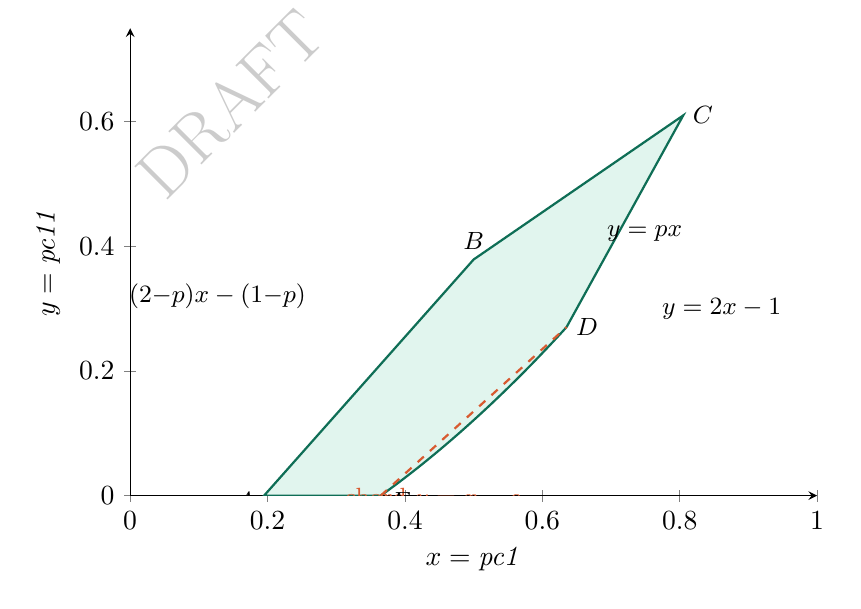
\begin{tikzpicture}
\begin{axis}[width=0.85\textwidth, height=0.62\textwidth,
  xlabel={$x=\mathit{pc1}$}, ylabel={$y=\mathit{pc11}$},
  xmin=0, xmax=1, ymin=0, ymax=0.75, axis lines=left,
  xtick={0,0.2,...,1}, ytick={0,0.2,0.4,0.6}]
\addplot[fill=regfill, draw=regline, thick] coordinates {(0.19494,0.00000) (0.50000,0.37893) (0.80506,0.61012) (0.63518,0.27037) (0.63068,0.26492) (0.62617,0.25950) (0.62166,0.25412) (0.61716,0.24878) (0.61265,0.24347) (0.60815,0.23819) (0.60364,0.23294) (0.59913,0.22773) (0.59463,0.22255) (0.59012,0.21740) (0.58562,0.21228) (0.58111,0.20720) (0.57660,0.20215) (0.57210,0.19713) (0.56759,0.19214) (0.56309,0.18718) (0.55858,0.18226) (0.55407,0.17737) (0.54957,0.17250) (0.54506,0.16767) (0.54055,0.16287) (0.53605,0.15811) (0.53154,0.15337) (0.52704,0.14866) (0.52253,0.14399) (0.51802,0.13934) (0.51352,0.13473) (0.50901,0.13014) (0.50451,0.12559) (0.50000,0.12107) (0.49549,0.11658) (0.49099,0.11212) (0.48648,0.10769) (0.48198,0.10329) (0.47747,0.09893) (0.47296,0.09459) (0.46846,0.09028) (0.46395,0.08601) (0.45945,0.08176) (0.45494,0.07755) (0.45043,0.07337) (0.44593,0.06922) (0.44142,0.06510) (0.43691,0.06101) (0.43241,0.05696) (0.42790,0.05293) (0.42340,0.04894) (0.41889,0.04498) (0.41438,0.04105) (0.40988,0.03715) (0.40537,0.03329) (0.40087,0.02946) (0.39636,0.02566) (0.39185,0.02189) (0.38735,0.01816) (0.38284,0.01446) (0.37834,0.01080) (0.37383,0.00716) (0.36932,0.00356) (0.36482,0.00000) (0.19494,0.00000)} -- cycle;
\addplot[chord, thick, dashed] coordinates {(0.36479,0) (0.63521,0.27041)};
\node[anchor=east] at (axis cs:0.27,0.32) {\small $y=(2{-}p)x-(1{-}p)$};
\node[anchor=west] at (axis cs:0.68,0.42) {\small $y=px$};
\node[anchor=west] at (axis cs:0.76,0.30) {\small $y=2x-1$};
\node[anchor=north, chord] at (axis cs:0.44,0.028) {\small chord $y=x-c$};
\node[below left] at (axis cs:0.195,0.02) {\small $A$};
\node[above] at (axis cs:0.5,0.379) {\small $B$};
\node[right] at (axis cs:0.805,0.610) {\small $C$};
\node[right] at (axis cs:0.635,0.270) {\small $D$};
\node[below right] at (axis cs:0.365,0.02) {\small $E$};
\end{axis}
\end{tikzpicture}
\caption{Exact region $\mathcal{R}_{0.4}$ ($p=2^{-0.4}$): five-edge regime.
The DE edge is the convex ellipse arc $y=x-p\sqrt{x(1-x)}$; the dashed line
is the conservative slope-1 chord.}
\label{fig:h04}
\end{figure}

\begin{figure}[htbp]
\centering
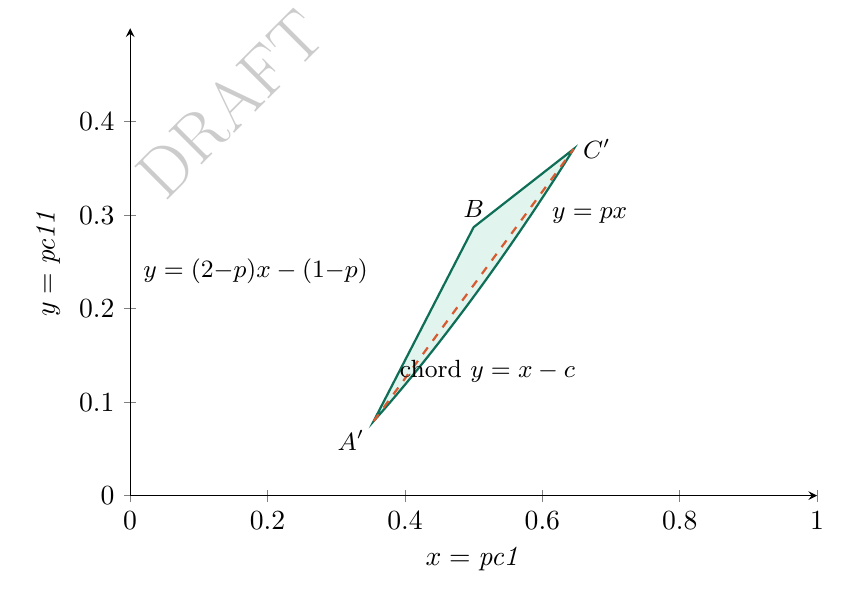
\begin{tikzpicture}
\begin{axis}[width=0.85\textwidth, height=0.62\textwidth,
  xlabel={$x=\mathit{pc1}$}, ylabel={$y=\mathit{pc11}$},
  xmin=0, xmax=1, ymin=0, ymax=0.5, axis lines=left,
  xtick={0,0.2,...,1}, ytick={0,0.1,...,0.4}]
\addplot[fill=regfill, draw=regline, thick] coordinates {(0.35452,0.07977) (0.50000,0.28717) (0.64548,0.37073) (0.64063,0.36505) (0.63578,0.35940) (0.63093,0.35378) (0.62608,0.34819) (0.62123,0.34263) (0.61639,0.33710) (0.61154,0.33160) (0.60669,0.32613) (0.60184,0.32068) (0.59699,0.31527) (0.59214,0.30988) (0.58729,0.30452) (0.58244,0.29920) (0.57759,0.29389) (0.57274,0.28862) (0.56789,0.28338) (0.56304,0.27816) (0.55819,0.27297) (0.55334,0.26781) (0.54849,0.26267) (0.54364,0.25757) (0.53880,0.25249) (0.53395,0.24743) (0.52910,0.24241) (0.52425,0.23741) (0.51940,0.23244) (0.51455,0.22750) (0.50970,0.22258) (0.50485,0.21769) (0.50000,0.21283) (0.49515,0.20799) (0.49030,0.20318) (0.48545,0.19840) (0.48060,0.19364) (0.47575,0.18892) (0.47090,0.18422) (0.46605,0.17954) (0.46120,0.17490) (0.45636,0.17028) (0.45151,0.16569) (0.44666,0.16112) (0.44181,0.15658) (0.43696,0.15208) (0.43211,0.14759) (0.42726,0.14314) (0.42241,0.13871) (0.41756,0.13432) (0.41271,0.12995) (0.40786,0.12561) (0.40301,0.12129) (0.39816,0.11701) (0.39331,0.11275) (0.38846,0.10853) (0.38361,0.10433) (0.37877,0.10016) (0.37392,0.09602) (0.36907,0.09191) (0.36422,0.08783) (0.35937,0.08379) (0.35452,0.07977)} -- cycle;
\addplot[chord, thick, dashed] coordinates {(0.35452,0.07977) (0.64548,0.37073)};
\node[anchor=east] at (axis cs:0.36,0.24) {\small $y=(2{-}p)x-(1{-}p)$};
\node[anchor=west] at (axis cs:0.60,0.30) {\small $y=px$};
\node[anchor=north] at (axis cs:0.52,0.155) {\small chord $y=x-c$};
\node[below left] at (axis cs:0.355,0.08) {\small $A'$};
\node[above] at (axis cs:0.5,0.287) {\small $B$};
\node[right] at (axis cs:0.645,0.371) {\small $C'$};
\end{axis}
\end{tikzpicture}
\caption{Exact region $\mathcal{R}_{0.8}$: triangle regime ($H>H^\ast$). The
region has detached from $y=0$ and from $y=2x-1$; only the two entropy lines
and the arc bind.}
\label{fig:h08}
\end{figure}

\begin{figure}[htbp]
\centering
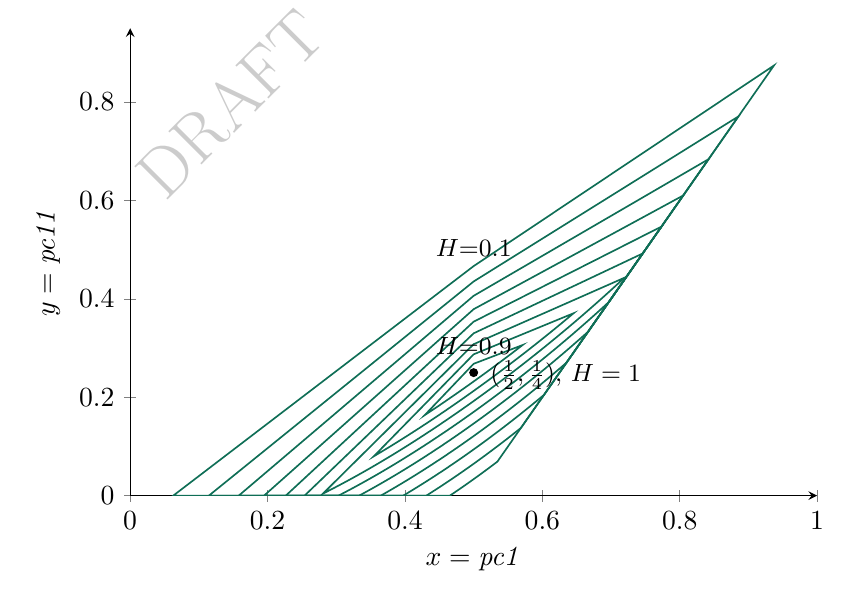
\begin{tikzpicture}
\begin{axis}[width=0.85\textwidth, height=0.62\textwidth,
  xlabel={$x=\mathit{pc1}$}, ylabel={$y=\mathit{pc11}$},
  xmin=0, xmax=1, ymin=0, ymax=0.95, axis lines=left,
  xtick={0,0.2,...,1}, ytick={0,0.2,...,0.8}]
\addplot[regline, semithick] coordinates {(0.06276,0.00000) (0.50000,0.46652) (0.93724,0.87447) (0.53460,0.06920) (0.53345,0.06798) (0.53230,0.06675) (0.53114,0.06553) (0.52999,0.06431) (0.52883,0.06309) (0.52768,0.06188) (0.52653,0.06067) (0.52537,0.05946) (0.52422,0.05825) (0.52307,0.05705) (0.52191,0.05585) (0.52076,0.05465) (0.51961,0.05345) (0.51845,0.05226) (0.51730,0.05106) (0.51615,0.04987) (0.51499,0.04869) (0.51384,0.04750) (0.51269,0.04632) (0.51153,0.04514) (0.51038,0.04396) (0.50923,0.04279) (0.50807,0.04162) (0.50692,0.04045) (0.50577,0.03928) (0.50461,0.03812) (0.50346,0.03695) (0.50231,0.03580) (0.50115,0.03464) (0.50000,0.03348) (0.49885,0.03233) (0.49769,0.03118) (0.49654,0.03003) (0.49539,0.02889) (0.49423,0.02775) (0.49308,0.02661) (0.49193,0.02547) (0.49077,0.02434) (0.48962,0.02320) (0.48847,0.02207) (0.48731,0.02095) (0.48616,0.01982) (0.48501,0.01870) (0.48385,0.01758) (0.48270,0.01646) (0.48155,0.01535) (0.48039,0.01423) (0.47924,0.01312) (0.47809,0.01202) (0.47693,0.01091) (0.47578,0.00981) (0.47463,0.00871) (0.47347,0.00761) (0.47232,0.00652) (0.47117,0.00542) (0.47001,0.00433) (0.46886,0.00325) (0.46770,0.00216) (0.46655,0.00108) (0.46540,0.00000) (0.06276,0.00000)} -- cycle;
\addplot[regline, semithick] coordinates {(0.11461,0.00000) (0.50000,0.43528) (0.88539,0.77077) (0.56887,0.13775) (0.56658,0.13518) (0.56428,0.13262) (0.56199,0.13007) (0.55969,0.12753) (0.55740,0.12500) (0.55510,0.12247) (0.55280,0.11996) (0.55051,0.11746) (0.54821,0.11496) (0.54592,0.11248) (0.54362,0.11000) (0.54132,0.10754) (0.53903,0.10508) (0.53673,0.10263) (0.53444,0.10020) (0.53214,0.09777) (0.52985,0.09535) (0.52755,0.09294) (0.52525,0.09053) (0.52296,0.08814) (0.52066,0.08576) (0.51837,0.08338) (0.51607,0.08102) (0.51377,0.07866) (0.51148,0.07632) (0.50918,0.07398) (0.50689,0.07165) (0.50459,0.06933) (0.50230,0.06703) (0.50000,0.06472) (0.49770,0.06243) (0.49541,0.06015) (0.49311,0.05788) (0.49082,0.05561) (0.48852,0.05336) (0.48623,0.05112) (0.48393,0.04888) (0.48163,0.04665) (0.47934,0.04443) (0.47704,0.04223) (0.47475,0.04003) (0.47245,0.03784) (0.47015,0.03566) (0.46786,0.03348) (0.46556,0.03132) (0.46327,0.02917) (0.46097,0.02702) (0.45868,0.02489) (0.45638,0.02276) (0.45408,0.02065) (0.45179,0.01854) (0.44949,0.01644) (0.44720,0.01436) (0.44490,0.01228) (0.44260,0.01021) (0.44031,0.00815) (0.43801,0.00610) (0.43572,0.00405) (0.43342,0.00202) (0.43113,0.00000) (0.11461,0.00000)} -- cycle;
\addplot[regline, semithick] coordinates {(0.15807,0.00000) (0.50000,0.40613) (0.84193,0.68386) (0.60250,0.20500) (0.59908,0.20101) (0.59567,0.19704) (0.59225,0.19309) (0.58883,0.18917) (0.58542,0.18526) (0.58200,0.18137) (0.57858,0.17750) (0.57517,0.17366) (0.57175,0.16983) (0.56833,0.16602) (0.56492,0.16223) (0.56150,0.15846) (0.55808,0.15471) (0.55467,0.15097) (0.55125,0.14726) (0.54783,0.14357) (0.54442,0.13990) (0.54100,0.13624) (0.53758,0.13261) (0.53417,0.12899) (0.53075,0.12539) (0.52733,0.12181) (0.52392,0.11826) (0.52050,0.11472) (0.51708,0.11119) (0.51367,0.10769) (0.51025,0.10421) (0.50683,0.10074) (0.50342,0.09730) (0.50000,0.09387) (0.49658,0.09047) (0.49317,0.08708) (0.48975,0.08371) (0.48633,0.08036) (0.48292,0.07703) (0.47950,0.07372) (0.47608,0.07042) (0.47267,0.06715) (0.46925,0.06389) (0.46583,0.06066) (0.46242,0.05744) (0.45900,0.05424) (0.45558,0.05106) (0.45217,0.04790) (0.44875,0.04476) (0.44533,0.04164) (0.44192,0.03854) (0.43850,0.03546) (0.43508,0.03240) (0.43167,0.02935) (0.42825,0.02633) (0.42483,0.02332) (0.42142,0.02034) (0.41800,0.01737) (0.41458,0.01443) (0.41117,0.01150) (0.40775,0.00860) (0.40433,0.00571) (0.40092,0.00285) (0.39750,0.00000) (0.15807,0.00000)} -- cycle;
\addplot[regline, semithick] coordinates {(0.19494,0.00000) (0.50000,0.37893) (0.80506,0.61012) (0.63518,0.27037) (0.63068,0.26492) (0.62617,0.25950) (0.62166,0.25412) (0.61716,0.24878) (0.61265,0.24347) (0.60815,0.23819) (0.60364,0.23294) (0.59913,0.22773) (0.59463,0.22255) (0.59012,0.21740) (0.58562,0.21228) (0.58111,0.20720) (0.57660,0.20215) (0.57210,0.19713) (0.56759,0.19214) (0.56309,0.18718) (0.55858,0.18226) (0.55407,0.17737) (0.54957,0.17250) (0.54506,0.16767) (0.54055,0.16287) (0.53605,0.15811) (0.53154,0.15337) (0.52704,0.14866) (0.52253,0.14399) (0.51802,0.13934) (0.51352,0.13473) (0.50901,0.13014) (0.50451,0.12559) (0.50000,0.12107) (0.49549,0.11658) (0.49099,0.11212) (0.48648,0.10769) (0.48198,0.10329) (0.47747,0.09893) (0.47296,0.09459) (0.46846,0.09028) (0.46395,0.08601) (0.45945,0.08176) (0.45494,0.07755) (0.45043,0.07337) (0.44593,0.06922) (0.44142,0.06510) (0.43691,0.06101) (0.43241,0.05696) (0.42790,0.05293) (0.42340,0.04894) (0.41889,0.04498) (0.41438,0.04105) (0.40988,0.03715) (0.40537,0.03329) (0.40087,0.02946) (0.39636,0.02566) (0.39185,0.02189) (0.38735,0.01816) (0.38284,0.01446) (0.37834,0.01080) (0.37383,0.00716) (0.36932,0.00356) (0.36482,0.00000) (0.19494,0.00000)} -- cycle;
\addplot[regline, semithick] coordinates {(0.22654,0.00000) (0.50000,0.35355) (0.77346,0.54692) (0.66667,0.33333) (0.66111,0.32641) (0.65556,0.31955) (0.65000,0.31273) (0.64444,0.30597) (0.63889,0.29925) (0.63333,0.29258) (0.62778,0.28596) (0.62222,0.27939) (0.61667,0.27287) (0.61111,0.26640) (0.60556,0.25997) (0.60000,0.25359) (0.59444,0.24726) (0.58889,0.24097) (0.58333,0.23472) (0.57778,0.22853) (0.57222,0.22238) (0.56667,0.21627) (0.56111,0.21021) (0.55556,0.20419) (0.55000,0.19822) (0.54444,0.19229) (0.53889,0.18641) (0.53333,0.18057) (0.52778,0.17477) (0.52222,0.16902) (0.51667,0.16331) (0.51111,0.15765) (0.50556,0.15202) (0.50000,0.14645) (0.49444,0.14091) (0.48889,0.13542) (0.48333,0.12998) (0.47778,0.12457) (0.47222,0.11921) (0.46667,0.11390) (0.46111,0.10863) (0.45556,0.10340) (0.45000,0.09822) (0.44444,0.09308) (0.43889,0.08799) (0.43333,0.08294) (0.42778,0.07793) (0.42222,0.07297) (0.41667,0.06806) (0.41111,0.06319) (0.40556,0.05837) (0.40000,0.05359) (0.39444,0.04886) (0.38889,0.04418) (0.38333,0.03954) (0.37778,0.03495) (0.37222,0.03041) (0.36667,0.02592) (0.36111,0.02147) (0.35556,0.01708) (0.35000,0.01273) (0.34444,0.00844) (0.33889,0.00419) (0.33333,0.00000) (0.22654,0.00000)} -- cycle;
\addplot[regline, semithick] coordinates {(0.25387,0.00000) (0.50000,0.32988) (0.74613,0.49226) (0.69673,0.39346) (0.69017,0.38509) (0.68362,0.37679) (0.67706,0.36856) (0.67050,0.36039) (0.66394,0.35230) (0.65738,0.34428) (0.65083,0.33632) (0.64427,0.32842) (0.63771,0.32059) (0.63115,0.31283) (0.62460,0.30513) (0.61804,0.29749) (0.61148,0.28991) (0.60492,0.28239) (0.59837,0.27493) (0.59181,0.26754) (0.58525,0.26020) (0.57869,0.25293) (0.57213,0.24571) (0.56558,0.23855) (0.55902,0.23145) (0.55246,0.22441) (0.54590,0.21742) (0.53935,0.21049) (0.53279,0.20362) (0.52623,0.19681) (0.51967,0.19005) (0.51312,0.18335) (0.50656,0.17671) (0.50000,0.17012) (0.49344,0.16359) (0.48688,0.15712) (0.48033,0.15071) (0.47377,0.14435) (0.46721,0.13804) (0.46065,0.13180) (0.45410,0.12561) (0.44754,0.11948) (0.44098,0.11341) (0.43442,0.10740) (0.42787,0.10144) (0.42131,0.09554) (0.41475,0.08970) (0.40819,0.08392) (0.40163,0.07820) (0.39508,0.07254) (0.38852,0.06695) (0.38196,0.06141) (0.37540,0.05593) (0.36885,0.05052) (0.36229,0.04517) (0.35573,0.03988) (0.34917,0.03466) (0.34262,0.02951) (0.33606,0.02442) (0.32950,0.01939) (0.32294,0.01444) (0.31638,0.00956) (0.30983,0.00474) (0.30327,0.00000) (0.25387,0.00000)} -- cycle;
\addplot[regline, semithick] coordinates {(0.28058,0.00401) (0.50000,0.30779) (0.71942,0.44286) (0.71211,0.43339) (0.70479,0.42401) (0.69748,0.41472) (0.69017,0.40551) (0.68285,0.39638) (0.67554,0.38734) (0.66822,0.37838) (0.66091,0.36950) (0.65359,0.36069) (0.64628,0.35196) (0.63897,0.34331) (0.63165,0.33473) (0.62434,0.32622) (0.61702,0.31779) (0.60971,0.30943) (0.60240,0.30113) (0.59508,0.29291) (0.58777,0.28476) (0.58045,0.27668) (0.57314,0.26867) (0.56583,0.26072) (0.55851,0.25284) (0.55120,0.24503) (0.54388,0.23729) (0.53657,0.22961) (0.52926,0.22200) (0.52194,0.21445) (0.51463,0.20697) (0.50731,0.19956) (0.50000,0.19221) (0.49269,0.18493) (0.48537,0.17772) (0.47806,0.17057) (0.47074,0.16349) (0.46343,0.15647) (0.45612,0.14952) (0.44880,0.14263) (0.44149,0.13582) (0.43417,0.12907) (0.42686,0.12238) (0.41955,0.11577) (0.41223,0.10922) (0.40492,0.10275) (0.39760,0.09634) (0.39029,0.09000) (0.38298,0.08374) (0.37566,0.07754) (0.36835,0.07142) (0.36103,0.06537) (0.35372,0.05940) (0.34641,0.05350) (0.33909,0.04768) (0.33178,0.04193) (0.32446,0.03627) (0.31715,0.03068) (0.30983,0.02518) (0.30252,0.01976) (0.29521,0.01442) (0.28789,0.00917) (0.28058,0.00401)} -- cycle;
\addplot[regline, semithick] coordinates {(0.35452,0.07977) (0.50000,0.28717) (0.64548,0.37073) (0.64063,0.36505) (0.63578,0.35940) (0.63093,0.35378) (0.62608,0.34819) (0.62123,0.34263) (0.61639,0.33710) (0.61154,0.33160) (0.60669,0.32613) (0.60184,0.32068) (0.59699,0.31527) (0.59214,0.30988) (0.58729,0.30452) (0.58244,0.29920) (0.57759,0.29389) (0.57274,0.28862) (0.56789,0.28338) (0.56304,0.27816) (0.55819,0.27297) (0.55334,0.26781) (0.54849,0.26267) (0.54364,0.25757) (0.53880,0.25249) (0.53395,0.24743) (0.52910,0.24241) (0.52425,0.23741) (0.51940,0.23244) (0.51455,0.22750) (0.50970,0.22258) (0.50485,0.21769) (0.50000,0.21283) (0.49515,0.20799) (0.49030,0.20318) (0.48545,0.19840) (0.48060,0.19364) (0.47575,0.18892) (0.47090,0.18422) (0.46605,0.17954) (0.46120,0.17490) (0.45636,0.17028) (0.45151,0.16569) (0.44666,0.16112) (0.44181,0.15658) (0.43696,0.15208) (0.43211,0.14759) (0.42726,0.14314) (0.42241,0.13871) (0.41756,0.13432) (0.41271,0.12995) (0.40786,0.12561) (0.40301,0.12129) (0.39816,0.11701) (0.39331,0.11275) (0.38846,0.10853) (0.38361,0.10433) (0.37877,0.10016) (0.37392,0.09602) (0.36907,0.09191) (0.36422,0.08783) (0.35937,0.08379) (0.35452,0.07977)} -- cycle;
\addplot[regline, semithick] coordinates {(0.42859,0.16340) (0.50000,0.26794) (0.57141,0.30621) (0.56903,0.30365) (0.56665,0.30109) (0.56427,0.29854) (0.56188,0.29600) (0.55950,0.29347) (0.55712,0.29094) (0.55474,0.28841) (0.55236,0.28589) (0.54998,0.28338) (0.54760,0.28088) (0.54522,0.27838) (0.54284,0.27589) (0.54046,0.27340) (0.53808,0.27092) (0.53570,0.26844) (0.53332,0.26597) (0.53094,0.26351) (0.52856,0.26106) (0.52618,0.25861) (0.52380,0.25616) (0.52142,0.25372) (0.51904,0.25129) (0.51666,0.24887) (0.51428,0.24645) (0.51190,0.24403) (0.50952,0.24163) (0.50714,0.23922) (0.50476,0.23683) (0.50238,0.23444) (0.50000,0.23206) (0.49762,0.22968) (0.49524,0.22731) (0.49286,0.22494) (0.49048,0.22258) (0.48810,0.22023) (0.48572,0.21788) (0.48334,0.21554) (0.48096,0.21321) (0.47858,0.21088) (0.47620,0.20856) (0.47382,0.20624) (0.47144,0.20393) (0.46906,0.20163) (0.46668,0.19933) (0.46430,0.19704) (0.46192,0.19475) (0.45954,0.19247) (0.45716,0.19020) (0.45478,0.18793) (0.45240,0.18567) (0.45002,0.18341) (0.44764,0.18117) (0.44526,0.17892) (0.44288,0.17669) (0.44050,0.17446) (0.43812,0.17223) (0.43573,0.17001) (0.43335,0.16780) (0.43097,0.16560) (0.42859,0.16340)} -- cycle;
\addplot[only marks, mark=*, mark size=1.4pt, black] coordinates {(0.5,0.25)};
\node[right] at (axis cs:0.51,0.245) {\small $(\tfrac12,\tfrac14)$, $H=1$};
\node[above] at (axis cs:0.5,0.4665) {\small $H{=}0.1$};
\node[above] at (axis cs:0.5,0.267944) {\small $H{=}0.9$};
\end{axis}
\end{tikzpicture}
\caption{The nested family of exact boundaries for
$H=0.1,0.2,\dots,0.9$, shrinking onto the full-entropy point
$(\tfrac12,\tfrac14)$. Apex $B$ of each region lies on $x=\tfrac12$ at height
$p/2$; the structural transition from five edges to three occurs between
$H=0.6$ and $H=0.7$, at $H^\ast=\log_2\varphi$.}
\label{fig:nested}
\end{figure}

\section{The Conservative Chord for the Elliptic Arc}
\label{sec:chord}

\begin{proposition}[Slope-1 chord]
At every entropy level, the chord connecting the endpoints of the active arc
has slope exactly $1$. In the five-edge regime the endpoints are $E$ and $D$
and $D_x - E_x = \frac{1-p^2}{1+p^2} = D_y - E_y$; in the triangle regime the
endpoints are $A'$ and $C'$ and the same cancellation occurs. The chord is
\begin{equation}
y \;\ge\; x - c(H),\qquad
c(H) =
\begin{cases}
\dfrac{p^2}{1+p^2}, & H \le H^\ast,\\[8pt]
\dfrac{p^2(1-p)}{(1-p)^2+p^2}, & H > H^\ast.
\end{cases}
\label{eq:chord}
\end{equation}
\end{proposition}

Because the arc is convex and the chord endpoints lie on it, the chord lies
above the arc: requiring $y\ge x-c$ is strictly stronger than the exact arc
constraint, so replacing the arc with the chord yields a test that can only
reject data whose true entropy is $\ge H$, never accept data below it. The
chord is the only place the linear test gives anything away; the maximum
sagitta (at $x=\tfrac12$, five-edge regime) is $c(H)-\tfrac{1-p}{2}$, about
$0.014$ at $H=0.4$.

\section{Table of Linear Inequalities}
\label{sec:table}

Table~\ref{tab:ineq} lists the four linear tests at nine entropy levels.

\begin{table}[htbp]
\centering
\caption{Linear inequalities defining the conservative polygon at each
entropy threshold, with $p=2^{-H}$. The DC test is only an active boundary
edge for $H\le0.6$ of the listed levels; above $H^\ast$ it is implied by the
others (marked ---) but remains harmless to include.}
\label{tab:ineq}
\begin{tabular}{cccccc}
\toprule
$H$ & $p=2^{-H}$ & AB: $y\le$ & BC: $y\le$ & DC: $y\ge$ & ED chord: $y\ge$\\
\midrule
0.1 & 0.933033 & $1.066967x - 0.066967$ & $0.933033x$ & $2x-1$ & $x - 0.465398$\\
0.2 & 0.870551 & $1.129449x - 0.129449$ & $0.870551x$ & $2x-1$ & $x - 0.431126$\\
0.3 & 0.812252 & $1.187748x - 0.187748$ & $0.812252x$ & $2x-1$ & $x - 0.397501$\\
0.4 & 0.757858 & $1.242142x - 0.242142$ & $0.757858x$ & $2x-1$ & $x - 0.364817$\\
0.5 & 0.707107 & $1.292893x - 0.292893$ & $0.707107x$ & $2x-1$ & $x - 1/3$ (exact)\\
0.6 & 0.659754 & $1.340246x - 0.340246$ & $0.659754x$ & $2x-1$ & $x - 0.303269$\\
0.7 & 0.615572 & $1.384428x - 0.384428$ & $0.615572x$ & --- & $x - 0.276565$\\
0.8 & 0.574349 & $1.425651x - 0.425651$ & $0.574349x$ & --- & $x - 0.274750$\\
0.9 & 0.535887 & $1.464113x - 0.464113$ & $0.535887x$ & --- & $x - 0.265198$\\
\bottomrule
\end{tabular}
\end{table}

\subsection{Perfect fit in the sub-threshold rows}
For $H\le H^\ast$ the chord line $y=x-c$ crosses $y=0$ at $x=c=x_E$ exactly
and crosses the DC line $y=2x-1$ at $x=1-c=x_D$ exactly. Consequently the
five tests $\{$AB, BC, DC, chord, $y\ge0\}$ reproduce the exact corners
$A$--$E$ with no slack anywhere except along the arc itself. The entire
conservatism of the linear polygon test is the thin sliver between the chord
and the convex arc.

\subsection{The \texorpdfstring{$H=0.5$}{H=0.5} special case}
At $H=\tfrac12$, $p^2=\tfrac12$ exactly, so $c=1/3$ and $D=(\tfrac23,\tfrac13)$:
the chord test becomes $3\,\mathit{count11} \ge 3\,\mathit{count1} - N$,
pure shift-and-add with zero coefficient quantization. Moreover the
\emph{exact} arc test is dyadic at this level:
$2(\mathit{count1}-\mathit{count11})^2 \le \mathit{count1}\,(N-\mathit{count1})$,
with no approximation at all. $H=0.5$ is the natural threshold for a
6{:}1-extraction design where hardware cost is at an absolute premium.

\subsection{Conversion to counts and rounding direction}
Multiplying each inequality by $N$ converts $x\to\mathit{count1}$,
$y\to\mathit{count11}$. All four constraints become monotonically
\emph{stricter} as $p$ (or $c$) decreases: for AB,
$\partial_p[(2-p)x-(1-p)] = 1-x > 0$; BC and the chord are immediate.
Therefore quantizing every irrational coefficient by rounding \emph{down}
(and the subtracted intercept term up) shrinks the accept region and
guarantees one-sided behavior: the integer test can only reject data whose
true entropy is at least $H$.

\subsection{Tight triangle cases}
At high thresholds the region is a thin triangle with apex
$B=(\tfrac12,p/2)$; at $H=0.9$ the arc's sagitta is only ${\approx}0.003$, so
the chord-versus-arc distinction becomes negligible, but coefficient
quantization dominates: the fixed-point resolution of $p$ must be fine enough
that the rounded-inward triangle does not collapse to the empty set. Twelve
fractional bits suffice for $N=2303$ at $H=0.9$ (Section~\ref{sec:integer});
as $H\to1$ the region converges to the single point $(\tfrac12,\tfrac14)$,
i.e.\ $\mathit{count1}=N/2$, $\mathit{count11}=N/4$, as it must for full
entropy data.

\section{Deriving the Integer Comparator Constants}
\label{sec:integer}

Fix a block size $n$ (hence $N=n-1$) and a fixed-point scale $S=2^k$. The
four comparators, in two's complement arithmetic, are
\begin{align}
\text{AB:}\quad & 2^k\,\mathit{count11} \;\le\; A_1\,\mathit{count1} - A_0,
& A_1 &= \lfloor (2-p)\,S \rfloor,\;\; A_0 = \lceil (1-p)\,S\,N \rceil,
\label{eq:ab}\\
\text{BC:}\quad & 2^k\,\mathit{count11} \;\le\; B_1\,\mathit{count1},
& B_1 &= \lfloor p\,S \rfloor,
\label{eq:bc}\\
\text{DC:}\quad & \mathit{count11} \;\ge\; 2\,\mathit{count1} - N,
& & \text{(exact; active for } H\le H^\ast\text{)},
\label{eq:dc}\\
\text{ED:}\quad & \mathit{count11} \;\ge\; \mathit{count1} - C_0,
& C_0 &= \lfloor c(H)\,N \rfloor.
\label{eq:ed}
\end{align}
The multiplications by $2^k$ are realized in hardware as $k$-bit left
shifts, i.e.\ wiring, at zero gate cost. The chord needs no fixed point
at all because its slope is exactly~1.
Table~\ref{tab:constants} gives the constants for the $n=2304$ example
of~\cite{johnston2024} ($N=2303$, $k=12$, $S=4096$).

\begin{table}[htbp]
\centering
\caption{Integer comparator constants for $n=2304$, $k=12$. Note
$A_1+B_1=8191$ in every row: the two slopes are $2-p$ and $p$, both floored,
so they straddle $2S$ by exactly one LSB. $C_0$ at $H=0.5$ is
$\lfloor 2303/3\rfloor = 767$, the dyadic case.}
\label{tab:constants}
\begin{tabular}{ccccccc}
\toprule
$H$ & $A_1$ & $A_0$ & $B_1$ & $C_0$ & DC active? & bitwidth\\
\midrule
0.1 & 4370 & 631{,}706   & 3821 & 1071 & yes  & 20\\
0.2 & 4626 & 1{,}221{,}108 & 3565 & 992 & yes & 21\\
0.3 & 4865 & 1{,}771{,}040 & 3326 & 915 & yes & 21\\
0.4 & 5087 & 2{,}284{,}145 & 3104 & 840 & yes & 22\\
0.5 & 5295 & 2{,}762{,}888 & 2896 & 767 & yes & 22\\
0.6 & 5489 & 3{,}209{,}571 & 2702 & 698 & yes & 22\\
0.7 & 5670 & 3{,}626{,}342 & 2521 & 636 & implied & 22\\
0.8 & 5839 & 4{,}015{,}202 & 2352 & 632 & implied & 22\\
0.9 & 5997 & 4{,}378{,}022 & 2194 & 610 & implied & 23\\
\bottomrule
\end{tabular}
\end{table}

Bit widths: the left side $2^{12}\,\mathit{count11}$ reaches
$2303\cdot4096 = 9{,}433{,}088$ (24 bits); the AB right side peaks near the
same value and reaches $-A_0\approx-4.4\mathrm{M}$ for small
$\mathit{count1}$, so a 25-bit two's complement comparison covers all rows.
The constant multiplies $A_1\,\mathit{count1}$ and $B_1\,\mathit{count1}$
synthesize to roughly 5--7 shift-adds each in canonical-signed-digit form;
DC is a shift and the chord a subtract, keeping the full four-threshold test
in the same sub-1000-gate class as the original polygon
test~\cite{johnston2024}, now with provably one-sided thresholds.

As a spot check of tightness at the hardest level: at
$\mathit{count1}=1152$ ($x\approx0.5$), $H=0.9$ yields the integer accept
window $\mathit{count11}\in[542,617]$ against the exact real-valued window
$[540.7,\,617.1]$ --- one count of conservatism at the bottom, zero at the
top.

Listing~\ref{lst:gen} generates the constants for arbitrary $(H,n,k)$ with
the correct rounding directions. One numerical caveat: double-precision
evaluation of $p$ leaves ${\sim}2^{-52}$ of ambiguity, which matters only if
a product lands within that distance of an exact integer; none of the nine
rows above does, but for arbitrary parameters the floor/ceil operations
should be evaluated with guard digits (e.g.\ \texttt{mpmath} or MPFR) to make
them unambiguous.

\begin{lstlisting}[caption={Generator for the integer comparator constants.},
label={lst:gen}]
import math

PHI_INV = (math.sqrt(5) - 1) / 2          # golden ratio threshold p* = 1/phi

def polygon_constants(H, n, k=12):
    N, S = n - 1, 1 << k
    p  = 2.0 ** (-H)
    p2 = 2.0 ** (-2 * H)
    if p >= PHI_INV:                       # H <= log2(phi) ~ 0.6942
        c = p2 / (1.0 + p2)                # chord intercept, arc endpoints E,D
        dc_active = True
    else:                                  # triangle regime: arc endpoints A',C'
        c = p2 * (1.0 - p) / ((1.0 - p) ** 2 + p2)
        dc_active = False
    a0 = math.ceil((1.0 - p) * S * N)
    return {
        'A1': math.floor((2.0 - p) * S),   # AB: (count11<<k) <= A1*count1 - A0
        'A0': a0,
        'B1': math.floor(p * S),           # BC: (count11<<k) <= B1*count1
        'C0': math.floor(c * N),           # ED: count11 >= count1 - C0
        'DC': dc_active,                   # DC: count11 >= 2*count1 - N
        'BW': math.ceil(math.log(a0,2))+1  # required bitwidth for arithmetic
    }

for H in [0.1, 0.2, 0.3, 0.4, 0.5, 0.6, 0.7, 0.8, 0.9]:
    print(H, polygon_constants(H, 2304))
\end{lstlisting}

\section{Multiplier-Based Exact Test of the Elliptic Arc}
\label{sec:hardware}

Where two multipliers are affordable, the arc can be tested exactly rather
than by chord, buying back the ${\sim}1$-count conservatism. The constraint
$(x-y)^2 \le p^2 x(1-x)$ scales to counts as
\begin{equation}
2^k\bigl(\mathit{count1}-\mathit{count11}\bigr)^2
\;\;\le\;\;
P_2 \cdot \mathit{count1}\cdot\bigl(N-\mathit{count1}\bigr),
\qquad
P_2 = \lfloor p^2\, 2^k \rfloor,
\label{eq:arcint}
\end{equation}
where flooring $P_2$ is the conservative direction (smaller $p^2$ shrinks the
region). For $k=12$ the constants are $P_2 = 3565$, $3104$, $2702$, $2352$,
$2048$, $1783$, $1552$, $1351$, $1176$ for $H=0.1$--$0.9$; the $H=0.5$ value
is exactly $2048$, reducing the constant multiply to a shift with zero
quantization loss. Note $\mathit{count1}-\mathit{count11}$ is simply
$\mathit{count10}$, so the left operand is directly available if a 10-pair
counter exists.

For $n=2304$: $d=\mathit{count1}-\mathit{count11}\le 2303$ (12 bits),
$d^2\le 5.3\mathrm{M}$ (23 bits), left side $2^{12}d^2$ needs 35 bits;
$\mathit{count1}(N-\mathit{count1}) \le \lfloor N^2/4 \rfloor \approx
1.33\mathrm{M}$ (21 bits), and $P_2\cdot q \le 4096\cdot1.33\mathrm{M}$
(33 bits). A single 35-bit unsigned comparison completes the test. The
datapath (Figure~\ref{fig:hw}) is two subtractors, one $12\times12$ squarer,
one $12\times12$ multiplier, one constant multiplier (CSD shift-add network,
or a true multiplier if $H$ must be runtime-programmable), and a comparator.
The test fires once per $n$-bit block, so a single multiplier can be
time-shared across the three products at three cycles per block if area is
critical.

\begin{figure}[htbp]
\centering
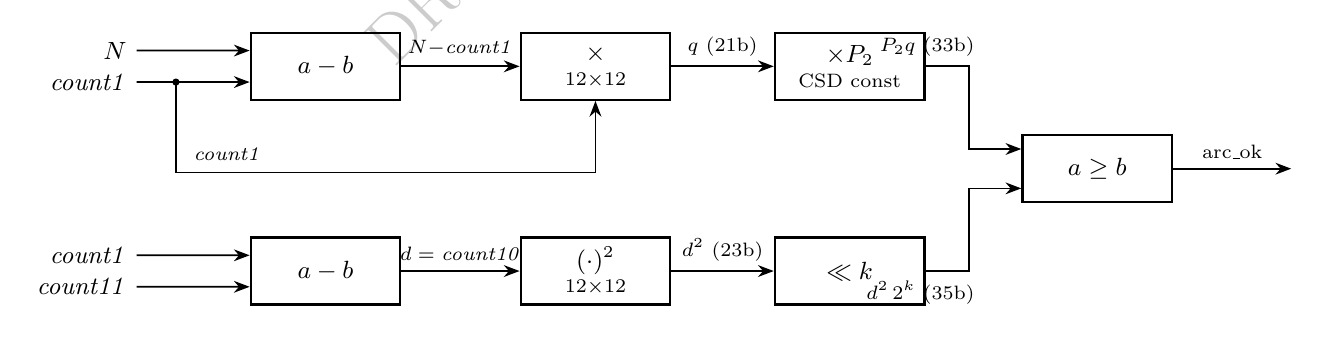
\begin{tikzpicture}[
  blk/.style={draw, thick, minimum width=1.9cm, minimum height=0.85cm, align=center, font=\small},
  wire/.style={-{Stealth[length=2mm]}, semithick},
  lbl/.style={font=\scriptsize}]
\node[blk] (sub1) at (0,0) {$a-b$};
\node[blk] (sub2) at (0,-2.6) {$a-b$};
\node[blk, right=1.5cm of sub1] (mul2) {$\times$\\[-2pt]{\scriptsize $12{\times}12$}};
\node[blk, right=1.5cm of sub2] (sq) {$(\cdot)^2$\\[-2pt]{\scriptsize $12{\times}12$}};
\node[blk, right=1.3cm of mul2] (cmul) {$\times P_2$\\[-2pt]{\scriptsize CSD const}};
\node[blk, right=1.3cm of sq] (shift) {$\ll k$};
\node[blk] (cmp) at (9.8,-1.3) {$a \ge b$};
\draw[wire] (-2.4,0.2) node[left, font=\small]{$N$} -- ([yshift=2mm]sub1.west);
\draw[wire] (-2.4,-0.2) node[left, font=\small]{$\mathit{count1}$} -- ([yshift=-2mm]sub1.west);
\draw[wire] (-2.4,-2.4) node[left, font=\small]{$\mathit{count1}$} -- ([yshift=2mm]sub2.west);
\draw[wire] (-2.4,-2.8) node[left, font=\small]{$\mathit{count11}$} -- ([yshift=-2mm]sub2.west);
\draw[wire] (sub1.east) -- node[lbl, above]{$N{-}\mathit{count1}$} (mul2.west);
\fill (-1.9,-0.2) circle (1.3pt);
\draw[wire] (-1.9,-0.2) -- (-1.9,-1.35) -| (mul2.south);
\node[lbl, anchor=south west] at (-1.8,-1.32) {$\mathit{count1}$};
\draw[wire] (sub2.east) -- node[lbl, above]{$d=\mathit{count10}$} (sq.west);
\draw[wire] (mul2.east) -- node[lbl, above]{$q$ (21b)} (cmul.west);
\draw[wire] (sq.east) -- node[lbl, above]{$d^2$ (23b)} (shift.west);
\draw[wire] (cmul.east) -- ++(0.55,0) node[lbl, above left, xshift=2mm]{$P_2 q$ (33b)} |- ([yshift=2.5mm]cmp.west);
\draw[wire] (shift.east) -- ++(0.55,0) node[lbl, below left, xshift=2mm]{$d^2\, 2^{k}$ (35b)} |- ([yshift=-2.5mm]cmp.west);
\draw[wire] (cmp.east) -- node[lbl, above]{arc\_ok} ++(1.5,0);
\end{tikzpicture}
\caption{Datapath for the exact elliptic-arc test
$2^k d^2 \le P_2\cdot \mathit{count1}\cdot(N-\mathit{count1})$ with
$d=\mathit{count1}-\mathit{count11}=\mathit{count10}$ and
$P_2=\lfloor p^2 2^k\rfloor$: two subtractors, one squarer, one multiplier,
one constant (CSD) multiplier, and a 35-bit comparator; the $\ll k$ block
denotes the $k$-bit left shift realizing the $2^k$ scaling as wiring. The
test fires once
per block, so the two array multipliers may be time-shared. At $H=0.5$,
$P_2=2^{k-1}$ and the constant multiplier reduces to a wire shift.}
\label{fig:hw}
\end{figure}

\section{Drawbacks and Scope}
\label{sec:drawbacks}

The limitations of~\cite{johnston2024} are inherited unchanged: the test
applies to single-bit-symbol sources whose statistics are captured by mean
and serial correlation, i.e.\ sources well modeled by the two-parameter
Markov chain; sources with longer-range structure (e.g.\ ring oscillators
with complex phase noise coupling) require different methods. The boundary
derived here is the \emph{asymptotic} rate boundary; for certification of
finite symbol widths $b$, the same three-pattern maximum applies with the
full MCV prefactors of~\cite{johnston2024}, shifting each edge by $O(1/b)$.
Finally, the counts over a finite block are estimates of $(x,y)$; the
statistical false-positive rate of the online test at a given block size is
set by the sampling distribution of the counts near the boundary, exactly as
for the graphically derived polygon, and is unchanged by this work --- what
changes is that the deterministic component of the error (boundary placement)
is eliminated.

\section{Conclusion}

A complete closed for description of the polygon test boundary from 
\cite{johnston2024} is derived.

The region of $(\mathit{count1},\mathit{count11})$ pairs with min-entropy rate at
least $H$ is bounded by the two lines $y\le px$ and $y\le(2-p)x-(1-p)$,
the line $y\ge 2x-1$ when $H\le\log_2\varphi$) and one curved edge that is
a convex arc of an ellipse $(x-y)^2=p^2x(1-x)$.

All corners have closed forms. A chord used as an easily computed approximation
to the arc has slope exactly~1 with intercept $c(H)$ given in equation~\eqref{eq:chord}.

An efficient two multiplier structure is given to identify points inside the arc
but outside the chord approximation.

By rounding integer constants toward the interior of the polygon yields a hardware test with only one-sided error. The uncertainty inherent in the image-extraction used in \cite{johnston2024} is eliminated while not increasing the gate count of digital hardware
implementations of the test.


\begin{thebibliography}{9}
\bibitem{johnston2024}
Johnston, D.: Online Testing Entropy and Entropy Tests with a Two State
Markov Model. In: Proceedings of SPACE 2024. Springer (2024)

\end{thebibliography}

\end{document}
